\documentclass{standalone}
\usepackage{tikz}
\usepackage{ctex,siunitx}
\usepackage{tkz-euclide}
\usepackage{amsmath}
\usetikzlibrary{patterns, calc}
\usetikzlibrary {decorations.pathmorphing, decorations.pathreplacing, decorations.shapes,}
\begin{document}
\small
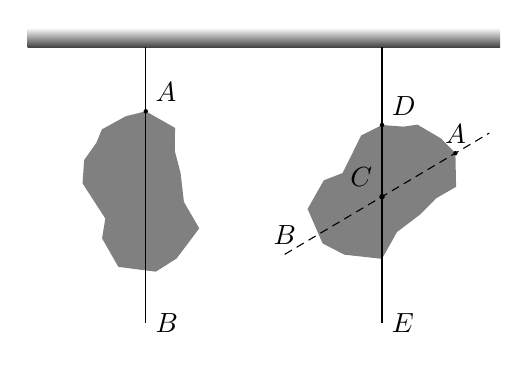
\begin{tikzpicture}[>=latex,scale=1]
  % \useasboundingbox (-0.1,0.1) rectangle(6,-3);
  \fill[top color=white,bottom color=darkgray]
    (-3,3.5)rectangle(3,3.75);
  \fill [gray] 
  (-1.754,2.625)--(-2.058,2.458)--(-2.126,2.291)--(-2.283,2.068)--(-2.303,1.773)--(-2.014,1.326)--(-2.055,1.074)--(-1.848,0.712)--(-1.373,0.651)--(-1.109,0.818)--(-0.821,1.201)--(-1.016,1.538)--(-1.058,1.905)--(-1.132,2.186)--(-1.128,2.477)--(-1.500,2.688)--(-1.754,2.625)--cycle;
  \fill [gray]
( 2.249,2.343)--( 1.950,2.519)--( 1.772,2.493)--( 1.500,2.514)--( 1.236,2.381)--( 0.999,1.904)--( 0.761,1.811)--( 0.555,1.448)--( 0.746,1.009)--( 1.023,0.867)--( 1.500,0.814)--( 1.690,1.154)--( 1.985,1.378)--( 2.189,1.584)--( 2.441,1.729)--( 2.432,2.156)--( 2.249,2.343)--cycle;
  \draw(-1.5,3.5)--(-1.5,0)node[right]{$B$};
  \draw(1.5,3.5)--(1.5,0)node[right]{$E$};
  \draw[densely dashed](0.2647,0.8714)--(2.8626,2.4114)node[at start,above]{$B$};
  \fill (2.432,2.156)circle(.8pt)node[above]{$A$};
  \fill (-1.5,2.688)circle(.8pt)node[above right]{$A$};
  \fill (1.5,2.514)circle(.8pt)node[above right]{$D$};
  \fill(1.5,1.6037)circle(1pt)node[above left]{$C$};
\end{tikzpicture}
\end{document}